\documentclass[../main.tex]{subfiles}

\begin{document}

\section{Question 1} \label{sec:q1}

Design an FSM that can detect an \lstinline{input_sequence} of 5 consecutive ones. Assume that a new input comes at every clock cycle. The output \lstinline{detected} should be asserted at the same cycle when the 5th '1' is given to the input. It should remain asserted as long as the input remains '1'.

\begin{enumerate}
    \item What should be the type of FSM machine?
    \item Draw the state diagram for the FSM machine.
    \item Derive the next state logic using D flops.
    \item Model the logic that you derived in the previous part in SystemVerilog strucutally.
    \item Model the FSM in a behavioral manner with SystemVerilog.
    \item Verify both structural and behavioral models and compare their results and waveforms together in your report.
\end{enumerate}

\subsection*{Solution}

To implement the FSM we choose a Moore Machine. The output only depends on \textit{if we have seen at least five consecutive 1's}. With a Moore Machine we can simply define five states and assert the output as 1 in the last and sixth state. There is no reason to make the output depend directly on the input, and the Moore Machine gives a glitch-free, synchronized output in comparison to a Mealy Machine. The FSM is defined with states $S_0 \ldots S_5$ and shown in the diagram in \cref{fig:q1}.

\begin{figure}[h]
    \centering
    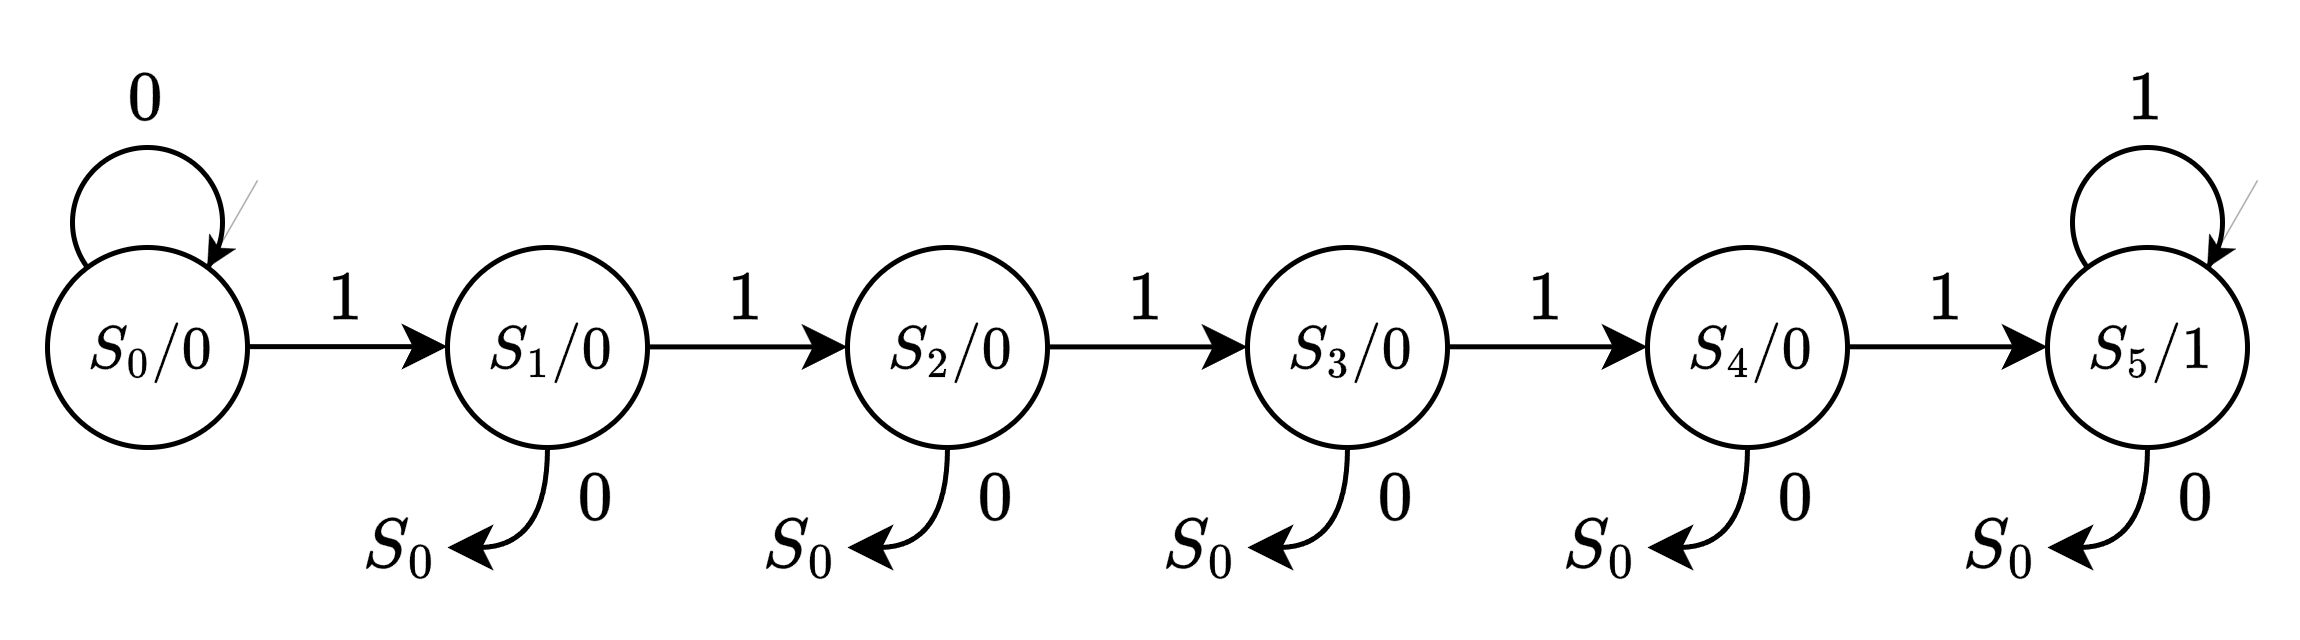
\includegraphics[width=\linewidth]{assets/q1_fsm.png}
    \caption{State transition diagram for sequence detector in Question 1.}
    \label{fig:q1}
\end{figure}

\begin{table}[h]
    \centering
    \begin{minipage}{0.48\textwidth}
        \centering
        \begin{tabular}{|c|c c|c|}
            \hline
            \textbf{State} & 0 & 1 & $w$ \\
            \hline
            $S_0$ & $S_0$ & $S_1$ & 0 \\
            $S_1$ & $S_0$ & $S_2$ & 0 \\
            $S_2$ & $S_0$ & $S_3$ & 0 \\
            $S_3$ & $S_0$ & $S_4$ & 0 \\
            $S_4$ & $S_0$ & $S_5$ & 0 \\
            $S_5$ & $S_0$ & $S_5$ & 1 \\
            \hline
            & \multicolumn{2}{|c|}{Next State} & \\
            \hline
        \end{tabular}
    \end{minipage}%
    \hspace{0.01\textwidth}
    \begin{minipage}{0.48\textwidth}
        \centering
        \begin{tabular}{|c|c c|c|}
            \hline
            $Q_2 Q_1 Q_0$ & 0 & 1 & $w$ \\
            \hline
            000 & 000 & 001 & 0 \\
            001 & 000 & 010 & 0 \\
            010 & 000 & 011 & 0 \\
            011 & 000 & 100 & 0 \\
            100 & 000 & 101 & 0 \\
            101 & 000 & 101 & 1 \\
            \hline
            & \multicolumn{2}{|c|}{$D_2 D_1 D_0$} & \\
            \hline
        \end{tabular}
    \end{minipage}
    \caption{State table (left) and transition table (right) for the sequence detector.}
    \label{tab:q1}
\end{table}

\newpage

Denoting each states bits $Q_0, Q_1, Q_2$, and their next state bits for $D_0, D_1, D_2$, the transition table is shown in \cref{tab:q1}. Denoting the input, $j$, Karnaugh maps for deducing logic expressions are shown below.

\begin{center}
    \begin{minipage}{0.45\textwidth}
        \centering
        \begin{karnaugh-map}[4][4][1][$j$][$Q_0$][$Q_1$][$Q_2$]
            \maxterms{0, 1, 2, 3, 4, 5, 6, 8, 10}
            \minterms{7, 9, 11}
            \indeterminants{12, 13, 14, 15}
            \implicant{13}{11}
            \implicant{7}{15}
        \end{karnaugh-map}

        \vspace{-40pt}
        \[
        D_2 = Q_1 Q_0 j + Q_2 j
        \]
    \end{minipage}%
    \begin{minipage}{0.45\textwidth}
        \centering
        \begin{karnaugh-map}[4][4][1][$j$][$Q_0$][$Q_1$][$Q_2$]
            \maxterms{0, 1, 2, 4, 6, 7, 8, 9, 10, 11}
            \minterms{3, 5}
            \indeterminants{12, 13, 14, 15}
            \implicant{5}{13}
            \implicant{3}{3}
        \end{karnaugh-map}

        \vspace{-40pt}
        \[
        D_1 = Q_1 \overline{Q_0} j + \overline{Q_2} \, \overline{Q_1} Q_0 j
        \]
    \end{minipage}
\end{center}

\begin{center}
    \begin{minipage}{0.45\textwidth}
        \centering
        \begin{karnaugh-map}[4][4][1][$j$][$Q_0$][$Q_1$][$Q_2$]
            \maxterms{0, 2, 3, 4, 6, 7, 8, 10}
            \minterms{1, 5, 9, 11}
            \indeterminants{12, 13, 14, 15}
            \implicant{1}{9}
            \implicant{13}{11}
        \end{karnaugh-map}

        \vspace{-40pt}
        \[
        D_0 = \overline{Q_0} j + Q_2 j
        \]
    \end{minipage}%
    \begin{minipage}{0.45\textwidth}
        \centering
        \begin{karnaugh-map}[4][2][1][$Q_0$][$Q_1$][$Q_2$]
            \maxterms{0, 1, 2, 3, 4}
            \minterms{5}
            \indeterminants{6, 7}
            \implicant{5}{7}
        \end{karnaugh-map}

        \vspace{-40pt}
        \[
        w = Q_2 Q_0
        \]
    \end{minipage}
\end{center}

\begin{figure}[h]
    \centering
    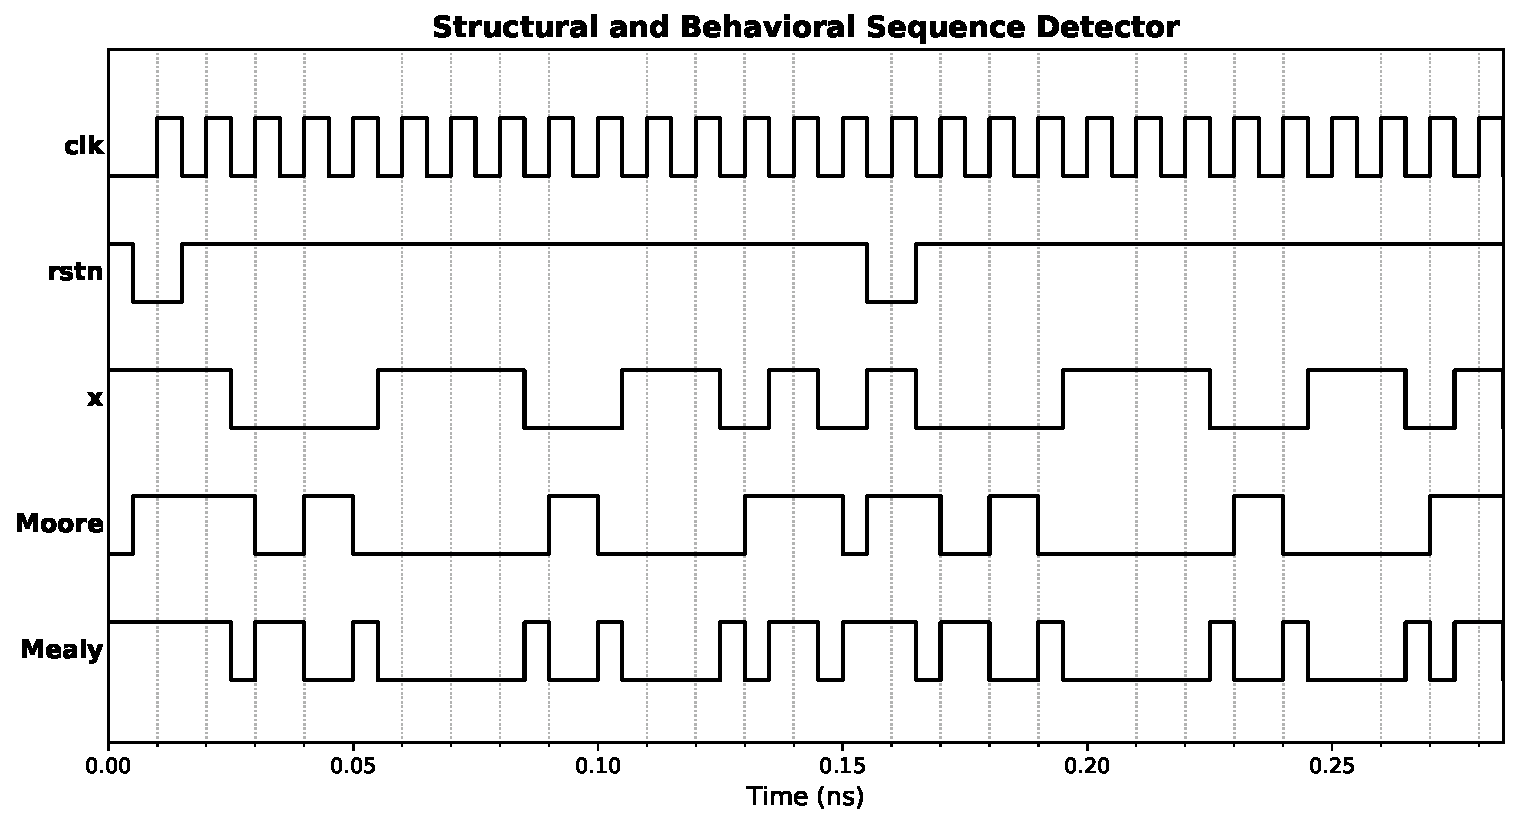
\includegraphics[width=0.9\textwidth]{assets/q1_wave.pdf}
    \caption{Waveforms for the structural and behavioral implementation.}
    \label{fig:q1_wave}
\end{figure}

\newpage

Using the found expressions for the next flip flop states, $D_0 \ldots D_2$, we can implement them directory in SystemVerilog to get the expected functionality. On a higher abstraction level, a behavioral implementation can be made, splitting the logic into a sequential \lstinline{always} block and a combination \lstinline{always} block. Both modules were verified simultaneously with the results shown in \cref{fig:q1_wave}. Implementations of both are shown in the following pages but can otherwise be found in:

\begin{itemize}
    \item \lstinline{hdl/q1/src/seq_detector_struct.sv}
    \item \lstinline{hdl/q1/src/seq_detector_behav.sv}
\end{itemize}

\begin{svminted}{Sequence Detector - Structural Implementation}
module seq_detector_struct (
    input   logic clk_i,
    input   logic rstn_i,
    input   logic seq_i,
    output  logic det_o
  );

  logic [2:0] Q;
  logic [2:0] D;

  assign D[2] = (Q[1] & Q[0] & seq_i) | (Q[2] & seq_i);
  assign D[1] = (Q[1] & ~Q[0] & seq_i) | (~Q[2] & ~Q[1] & Q[0] & seq_i);
  assign D[0] = (~Q[0] & seq_i) | Q[2] & seq_i;

  assign det_o = Q[2] & Q[0];

  always_ff @(posedge clk_i or negedge rstn_i) begin
    if (!rstn_i) begin
      Q <= 3'b000;
    end
    else begin
      Q <= D;
    end
  end

endmodule
\end{svminted}

\newpage

\begin{svminted}{Sequence Detector - Behavioral Implementation}
module seq_detector_behav (
    input   logic clk_i,
    input   logic rstn_i,
    input   logic seq_i,
    output  logic det_o
  );

  typedef enum logic [2:0] {
    S0,
    S1,
    S2,
    S3,
    S4,
    S5
  } state_t;

  state_t cur_state, nxt_state;

  always_ff @(posedge clk_i or negedge rstn_i) begin
    if (!rstn_i) begin
      cur_state <= S0;
    end
    else begin
      cur_state <= nxt_state;
    end
  end

  always_comb begin
    nxt_state = S0;

    case (cur_state)
      S0: nxt_state = seq_i ? S1 : S0;
      S1: nxt_state = seq_i ? S2 : S0;
      S2: nxt_state = seq_i ? S3 : S0;
      S3: nxt_state = seq_i ? S4 : S0;
      S4: nxt_state = seq_i ? S5 : S0;
      S5: nxt_state = seq_i ? S5 : S0;
      default: nxt_state = S0;
    endcase
  end

  assign det_o = (cur_state == S5) ? 1'b1 : 1'b0;

endmodule
\end{svminted}

\newpage

\section{Question 2}

Design a message conversion system with the conversion rule below:

For every cycle, if the input message bit is '0', toggle the current output bit; if the input message bit is '1', keep the output bit unchanged.

For example, let the input message be $x$, and the output message be $z$. Assuming $z$ initially is '1'. Given the sequence of $x = 10001110011010$, the output sequence of $z$ should be: 10100001000110. See the figure below.

\begin{figure}[h]
    \centering
    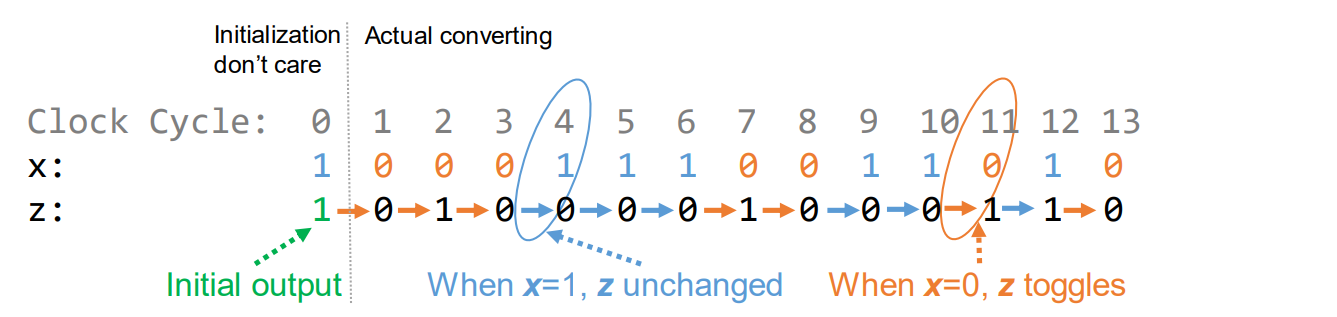
\includegraphics[width=\textwidth]{assets/q2.png}
\end{figure}

\begin{enumerate}
    \item Draw the state diagram of a \textbf{Mealy FSM} with the same behavior as described above.
    \item Draw the state diagram of a \textbf{Moore FSM} with the same behavior as described above.
    \item Model both FSMs in a behavioral manner using SystemVerilog.
    \item Write a testbench for both FSMs and compare the timing, number of states, and the output waveforms of Mealy and Moore FSMs in your report.
\end{enumerate}

\subsection*{Solution}

For a Moore Machine the output depends \textit{only} upon the current state. For a Mealy Machine the output depends on \textit{both} the current input and state. The state diagrams of the message conversion system implemented using both FSMs are shown in \cref{fig:q2_fsm}.

\vspace{-10pt}
\begin{figure}[h]
    \centering
    \begin{subfigure}{0.48\textwidth}
        \centering
        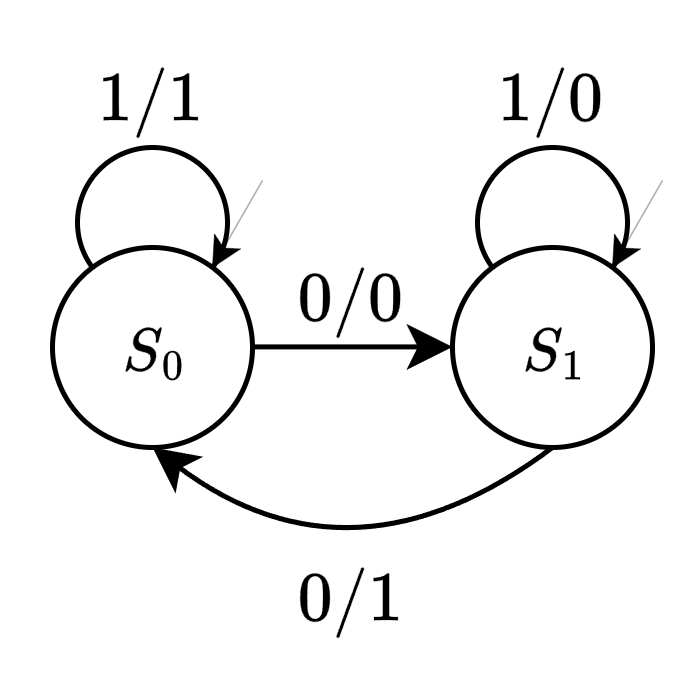
\includegraphics[width=0.8\textwidth]{assets/q2_mealy.png}
        \caption{Mealy FSM state diagram}
        \label{fig:q2_mealy}
    \end{subfigure}
    \hfill
    \begin{subfigure}{0.48\textwidth}
        \centering
        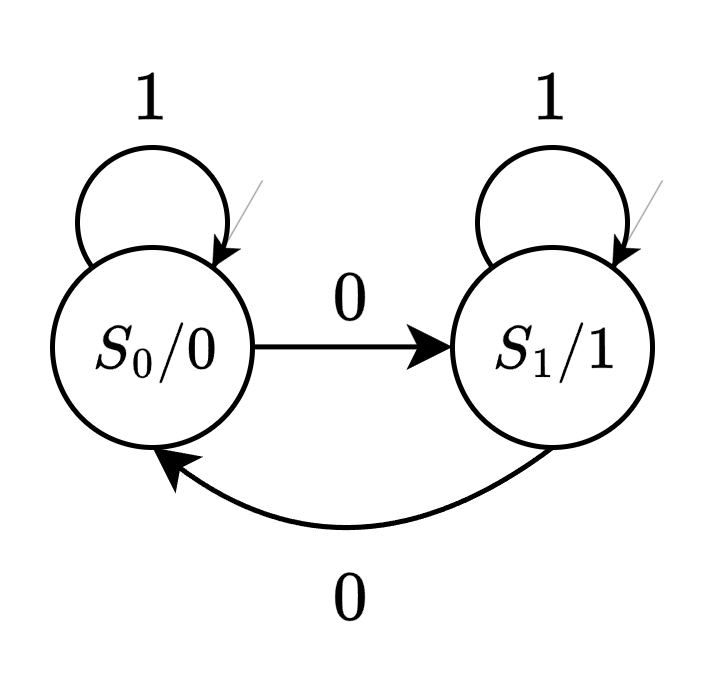
\includegraphics[width=0.8\textwidth]{assets/q2_moore.png}
        \caption{Moore FSM state diagram}
        \label{fig:q2_moore}
    \end{subfigure}
    \caption{State diagrams for the message conversion system using Mealy and Moore FSMs.}
    \label{fig:q2_fsm}
\end{figure}

\newpage

\begin{figure}[t]
    \centering
    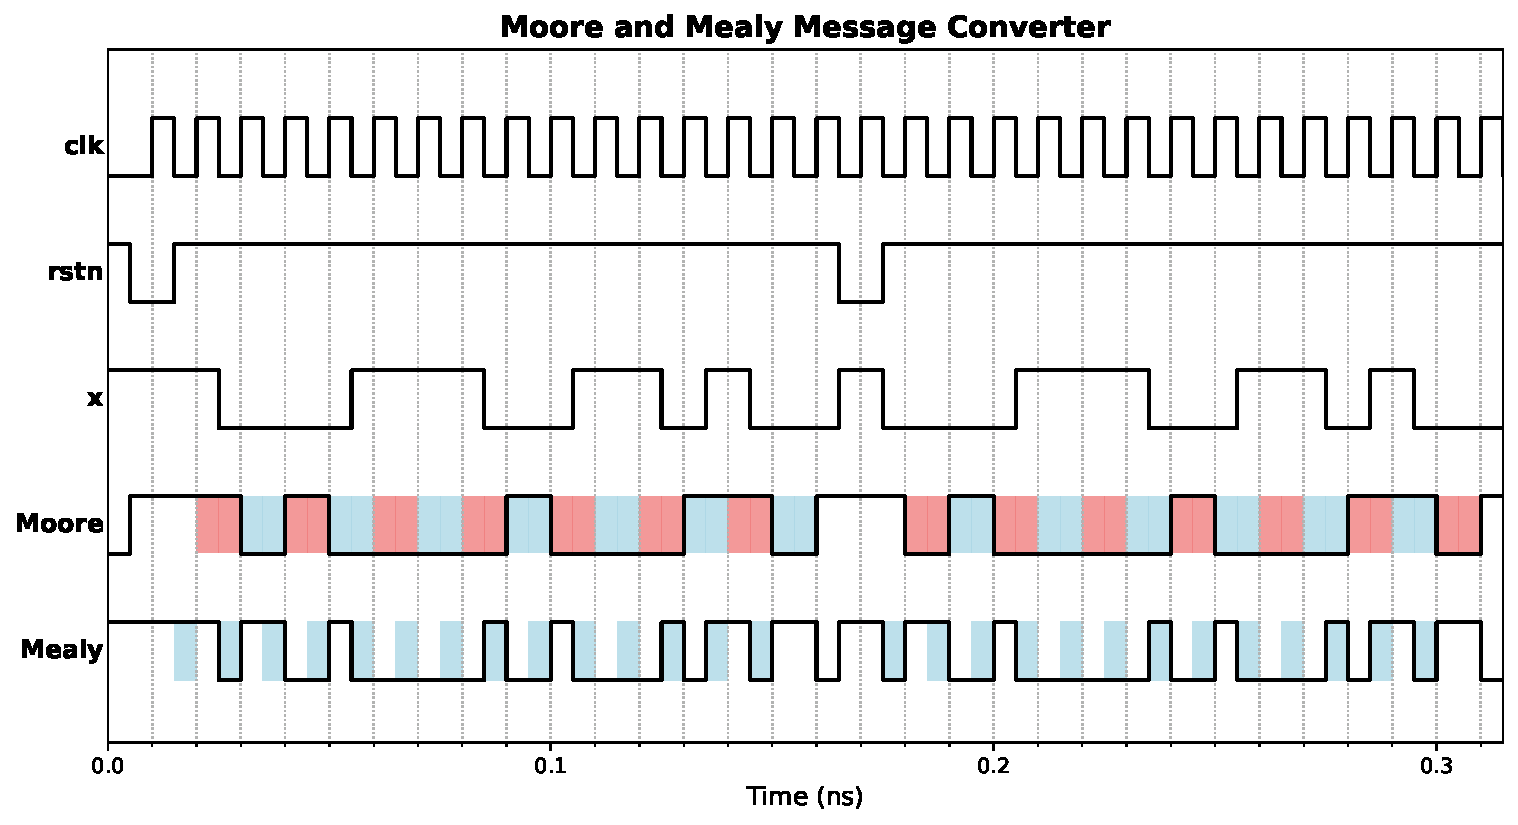
\includegraphics[width=\textwidth]{assets/q2_wave.pdf}
    \caption{Waveforms for the Moore and Mealy FSM implementations.}
    \label{fig:q2_wave}
\end{figure}

To compare the two FSMs, a testbench was written that writes the following test sequences, $x$, that has the expected outputs, $z$:

\begin{alignat*}{2}
    x &= \{ 1, 0, 0, 0, 1, 1, 1, 0, 0, 1, 1, 0, 1, 0 \}, 
    &\quad z &= \{ 1, 0, 1, 0, 0, 0, 0, 1, 0, 0, 0, 1, 1, 0 \} \\[6pt]
    x &= \{ 0, 0, 0, 1, 1, 1, 0, 0, 1, 1, 0, 1, 0 \}, 
    &\quad z &= \{ 0, 1, 0, 0, 0, 0, 1, 0, 0, 0, 1, 1, 0 \}
\end{alignat*}

The resulting waveforms are shown in \cref{fig:q2_wave}. Timing wise there is a significant difference between the two implementations as to when the output is valid. This is due to the Mealy Machine's combinational dependendency on the input, $x$. The waveforms for each FSM has been colored to illustrate when their outputs are valid. It is seen that both FSMs output the same sequences. The Moore Machine's output is always synchronized with the clock and is available for a full cycle. On the other hand, the Mealy Machine's output changes one half-cycle earlier and is only valid for half a cycle (on the rising edge).

In conclusion, both FSMs can be implemented using the same number of states, i.e. same number of memory elements. The Mealy Machine requries additional combinational logic but also makes it output available without any cycle delay. Behavioral implementations of both FSMs are shown in the following pages but can otherwise be found in:

\begin{itemize}
    \item \lstinline{hdl/q2/src/msg_converter_moore.sv}
    \item \lstinline{hdl/q2/src/msg_converter_mealy.sv}
\end{itemize}

\newpage

\begin{svminted}{Message Converter - Moore Implementation}
module msg_converter_moore (
    input   logic clk_i,
    input   logic rstn_i,
    input   logic x_i,
    output  logic z_o
  );

  typedef enum logic {
    S0,
    S1
  } state_t;

  state_t cur_state, nxt_state;

  always_ff @(posedge clk_i or negedge rstn_i) begin
    if (!rstn_i) begin
      cur_state <= S0;
    end
    else begin
      cur_state <= nxt_state;
    end
  end

  always_comb begin
    nxt_state = S0;

    case (cur_state)
      S0: nxt_state = x_i ? S0 : S1;
      S1: nxt_state = x_i ? S1 : S0;
      default: nxt_state = S0;
    endcase
  end

  assign z_o = (cur_state == S0) ? 1'b1 : 1'b0;

endmodule
\end{svminted}

\newpage

\begin{svminted}{Message Converter - Mealy Implementation}
module msg_converter_mealy (
    input   logic clk_i,
    input   logic rstn_i,
    input   logic x_i,
    output  logic z_o
  );

  typedef enum logic {
    S0,
    S1
  } state_t;

  state_t cur_state, nxt_state;

  always_ff @(posedge clk_i or negedge rstn_i) begin
    if (!rstn_i) begin
      cur_state <= S0;
    end
    else begin
      cur_state <= nxt_state;
    end
  end

  always_comb begin
    nxt_state = S0;
    case (cur_state)
      S0: nxt_state = x_i ? S0 : S1;
      S1: nxt_state = x_i ? S1 : S0;
    endcase
  end

  always_comb begin
    z_o = 1'b0;
    case (cur_state)
      S0: z_o = x_i ? 1'b1 : 1'b0;
      S1: z_o = x_i ? 1'b0 : 1'b1;
    endcase
  end

endmodule
\end{svminted}

\newpage

\section{Question 3}

A serial communication device has a begin-sequence (011010) that leads to the transmission of 32 bits on its \lstinline{serData} input. After receiving the begin-sequence, the \lstinline{outValid} output becomes 1, and the next 32 bits on \lstinline{serData} are regarded as valid serial data of the communication device. After 32 clock cycles, \lstinline{outValid} becomes 0 and the device returns to the first state, where it searches for the begin-sequence again.

\begin{enumerate}
    \item Create a state diagram to represent the Moore FSM for this system, clearly showing all states, transitions, and places where the output is issued. Draw the FSM in your report.
    \item Write a SystemVerilog description of this communication device, including the FSM and the counter.
    \item Write a testbench and verify the functionality of your design.
\end{enumerate}

\subsection*{Solution}

Much like in \cref{sec:q1} we design a sequence detector Moore FSM with seven states $S_0 \ldots S_6$. In the seventh state, $S_6$, a counter is enabled that counts 32 clock cycles and thereafter returns the FSM to $S_0$. By creating a 5-bit counter we can simply rely on overflow to reset the counter. The counter logic is implemented as an \lstinline{always_ff} block.

A testbench was written that inputs the sequence two times in a row to ensure the valid signal is triggered and held high for the specified 32 cycles, as well as ensuring that the counter reset logic works as expected. The waveforms are shown in \cref{fig:q3_wave}.

The implementation in SystemVerilog is shown in the following pages, but is otherwise found in:

\begin{itemize}
    \item \lstinline{hdl/q3/src/ser_comm.sv}
\end{itemize}

\begin{figure}[h]
    \centering
    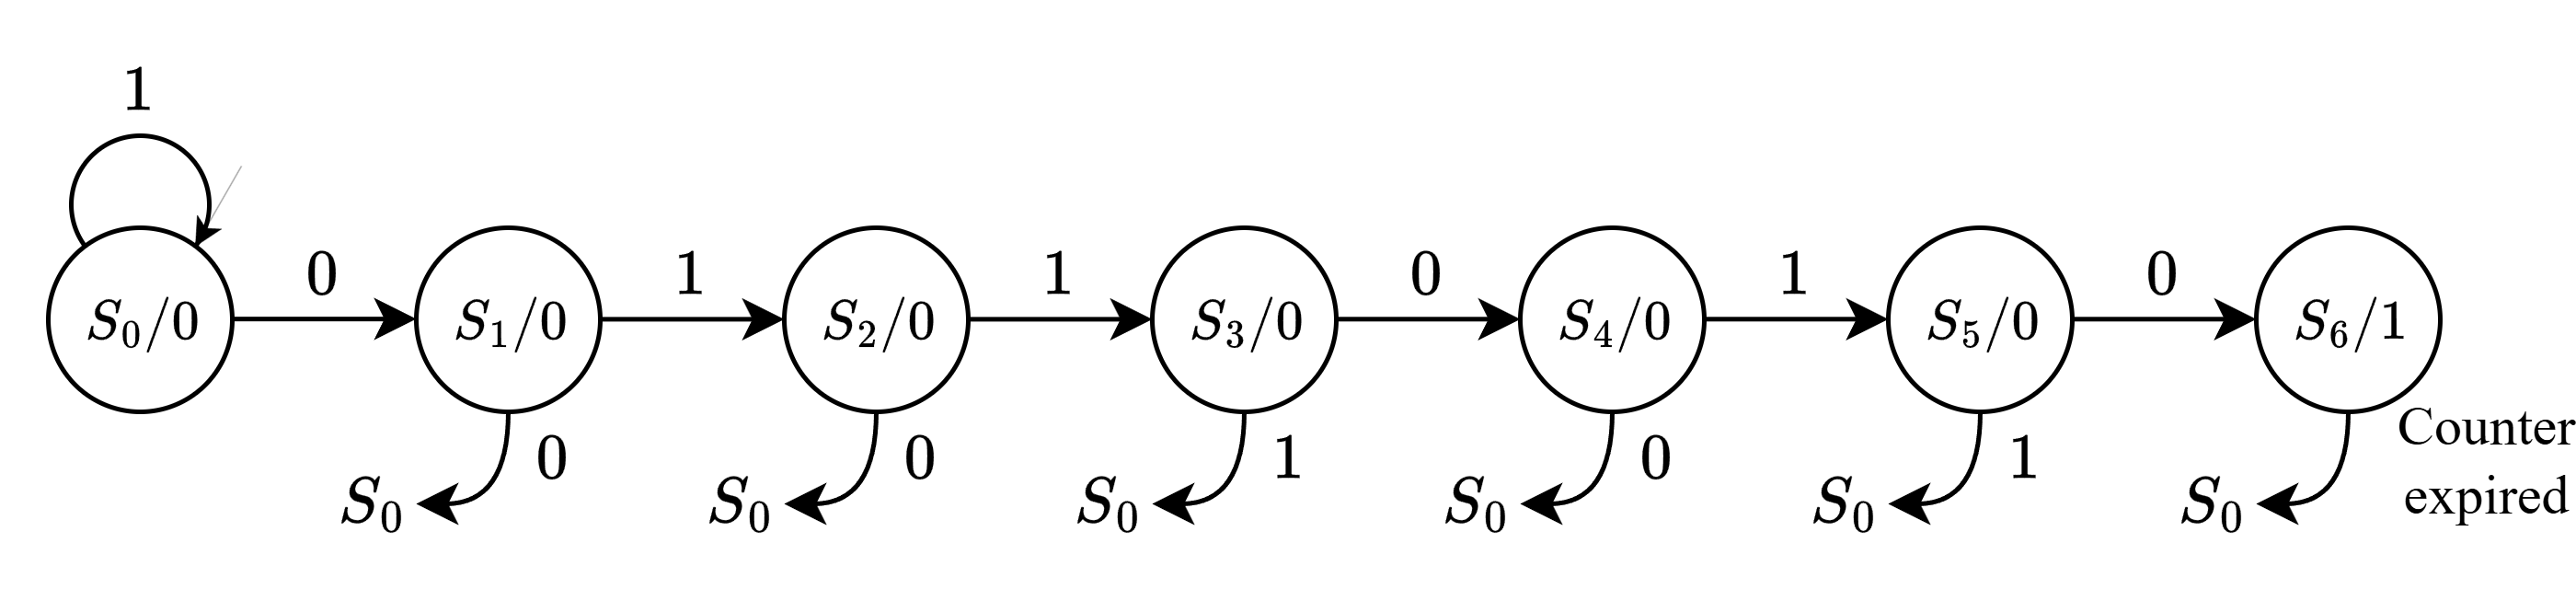
\includegraphics[width=\textwidth]{assets/q3_fsm.png}
    \caption{Moore FSM implementation of the serial communication device. State $S_6$ represents a counter active state that is left after 32 clock cycles.}
    \label{fig:q3_fsm}
\end{figure}

\newpage

\begin{figure}[h]
    \centering
    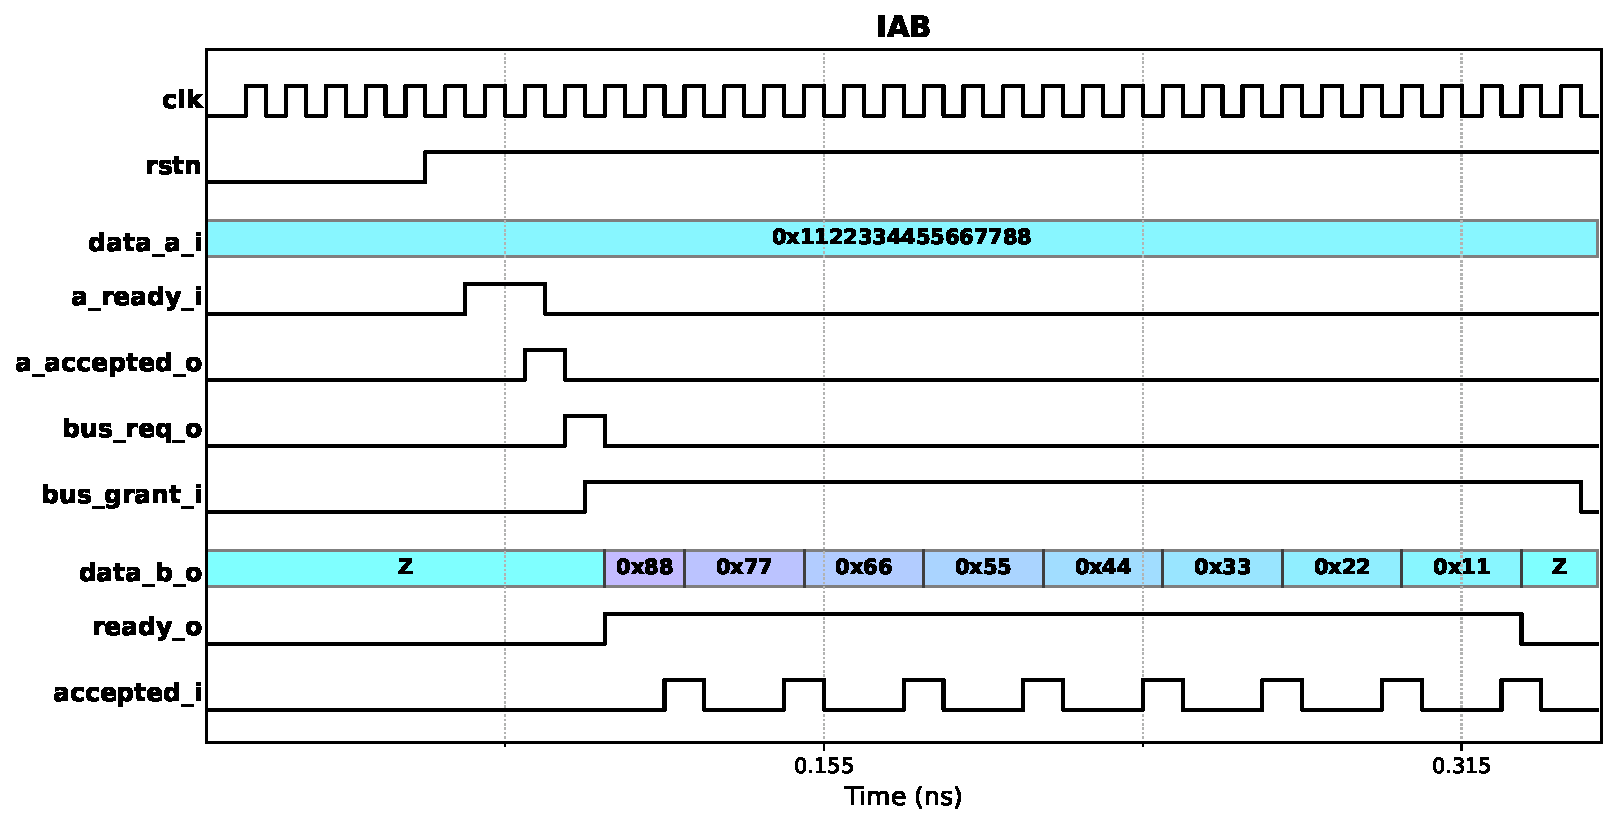
\includegraphics[width=\textwidth]{assets/q3_wave.pdf}
    \vspace{-10pt}
    \caption{Waveforms for the Moore FSM implementation of the serial communication sequence detector. After the specified begin-sequence has been detected, the valid signal is high for exactly 32 cycles (x-axis ticks are spaced by 8 cycles).}
    \label{fig:q3_wave}
\end{figure}

\begin{svminted}{Serial Communication Sequence Detector - Moore FSM}
module ser_comm (
    input   logic clk_i,
    input   logic rstn_i,
    input   logic serdata_i,
    output  logic valid_o
  );

  typedef enum logic [2:0] {S0, S1, S2, S3, S4, S5, S6} state_t;

  state_t cur_state, nxt_state;

  always_ff @(posedge clk_i or negedge rstn_i) begin
    if (!rstn_i) begin
      cur_state <= S0;
    end else begin
      cur_state <= nxt_state;
    end
  end

  always_comb begin
    nxt_state = S0;
    case (cur_state)
      S0: nxt_state = !serdata_i ? S1 : S0;
      S1: nxt_state =  serdata_i ? S2 : S0;
      S2: nxt_state =  serdata_i ? S3 : S0;
      S3: nxt_state = !serdata_i ? S4 : S0;
      S4: nxt_state =  serdata_i ? S5 : S0;
      S5: nxt_state = !serdata_i ? S6 : S0;
      S6: nxt_state = (counter == 5'b00000) ? S0 : S6;
      default: nxt_state = S0;
    endcase
  end

  logic [4:0] counter;
  always_ff @(posedge clk_i or negedge rstn_i) begin
    if (!rstn_i) begin
      counter <= 5'b11111;
    end else if (cur_state == S6) begin
      counter <= counter - 1;
    end
  end

  assign valid_o = (cur_state == S6) ? 1'b1 : 1'b0;

endmodule
\end{svminted}

\newpage

\section{Question 4}

Design and implement an \textit{average calculator} that computes the average of $n$ $m$-bit input numbers, where $n = 2^k$ with $k > 1$, and $m > 1$. The module should begin computation when it received a positive pulse on the start signal and assert the done signal once the average is ready.

\begin{enumerate}
    \item Draw a schematic of your datapath in your report, including the components, their interfaces, and necessary control signals.
    \item Draw a state diagram showing your controller's behavior in your report. In each state, show the control signals that are issued.
    \item Show the wiring between the datapath and controller within the top-level module in your report.
    \item Model the datapath and controller in SystemVerilog.
    \item Model the average calculator (top-level) by connecting the datapath and controller in SystemVerilog.
    \item Verify the fucntionality of your module with a testbench.
\end{enumerate}

\subsection*{Solution}

To calculate the average of $n$ $m$-bit inputs, we need to "accumulate" a sum, adding each value with the previous as they are clocked in. The final result can be computed combinatorially by dividing the sum by $n$. Since $n = 2^k, k > 1$ the division can be done by a right-shift operation, severely decreasing the hardware requirements.

The schematic is shown in \cref{fig:q4}. The datapath consists of an adder, register, and a divider module (right shifter). The datapath has two control signals it requires from the controller:

\begin{itemize}
    \item \textbf{en}: Enables new data to be clocked into the $m$-bit register/accumulator.
    \item \textbf{zero}: Zeroes the output of the $m$-bit register/accumulator to the adder. This way a cycle delay is avoided. 
\end{itemize}

The controller is designed as a Mealy Machine. This increases complexity compared to a Moore Machine but removes the intrinsic cycle delay and allows us to clock in the first input on the same cycle as \lstinline{start} is asserted. The transition diagram of the controller FSM is shown in \cref{fig:q4_controller}. To handle the full $m$-bit range of the input numbers we perform zero extension before adding them, and trim off the excess bits after division to have a $m$-bit output. A simple testbench was created that inputs two 4-bit sequences. The last sequence tests the input value boundary condition, ensuring that our bit-extension works. The resulting waveform is shown in \cref{fig:q4_wave}. The implementations in SystemVerilog can be found in:

\begin{itemize}
    \item \lstinline{hdl/q4/src/avg_calc.sv}
    \item \lstinline{hdl/q4/src/avg_calc_dp.sv}
    \item \lstinline{hdl/q4/src/avg_calc_controller.sv}
\end{itemize}

\newpage

\begin{figure}[H]
    \centering
    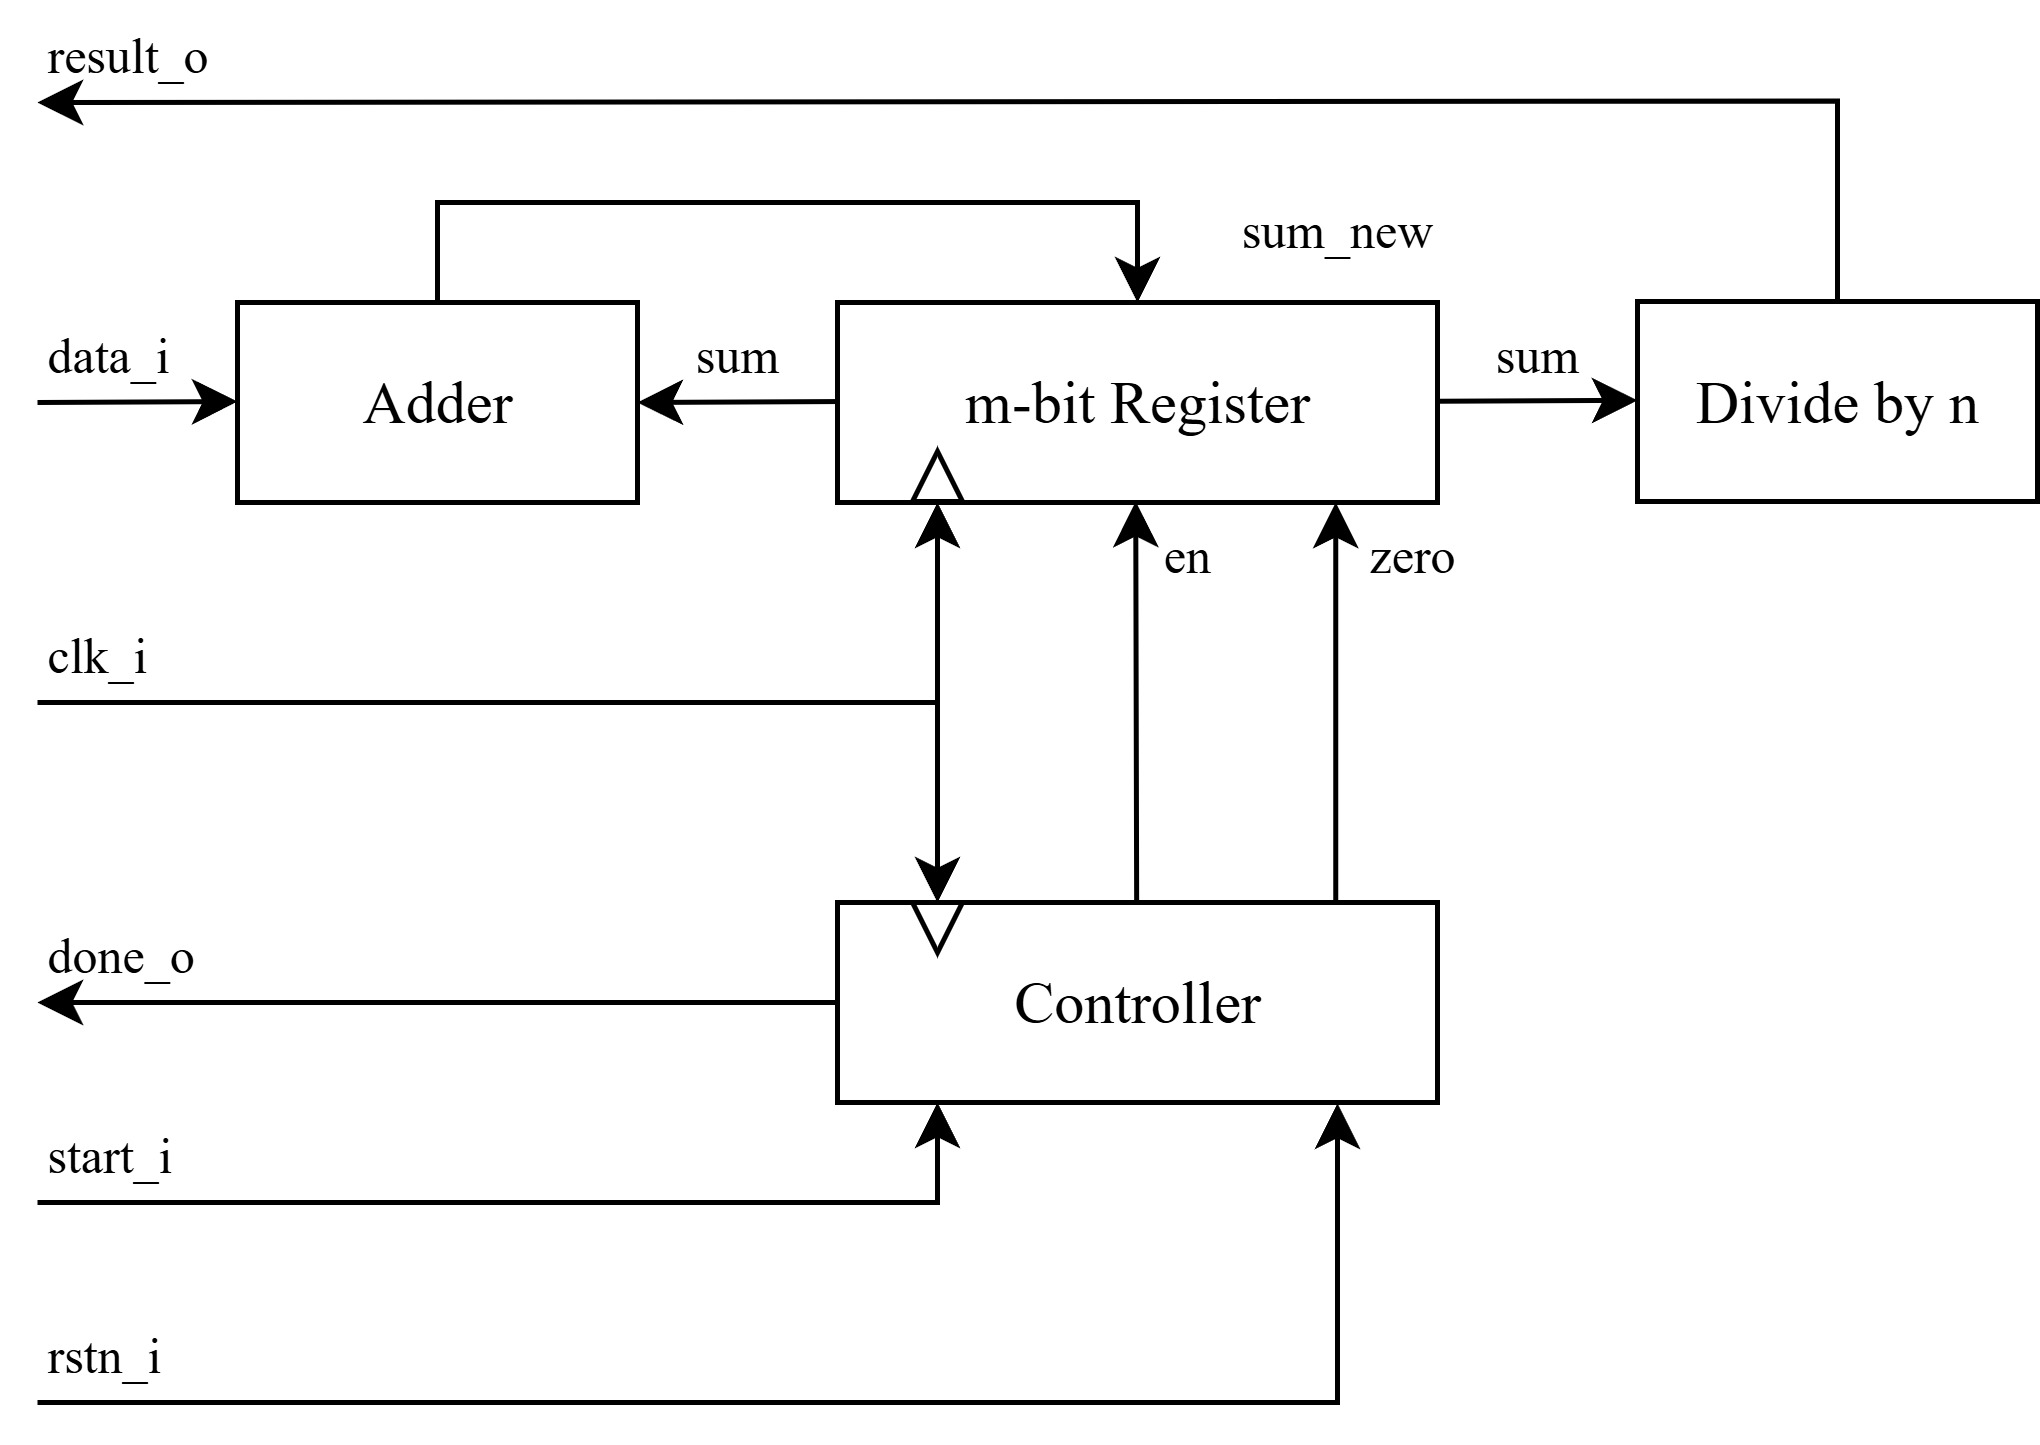
\includegraphics[width=0.9\textwidth]{assets/q4.png}
    \caption{Schematic of the \textit{average calculator} module.}
    \label{fig:q4}
\end{figure}


\begin{figure}[H]
    \centering
    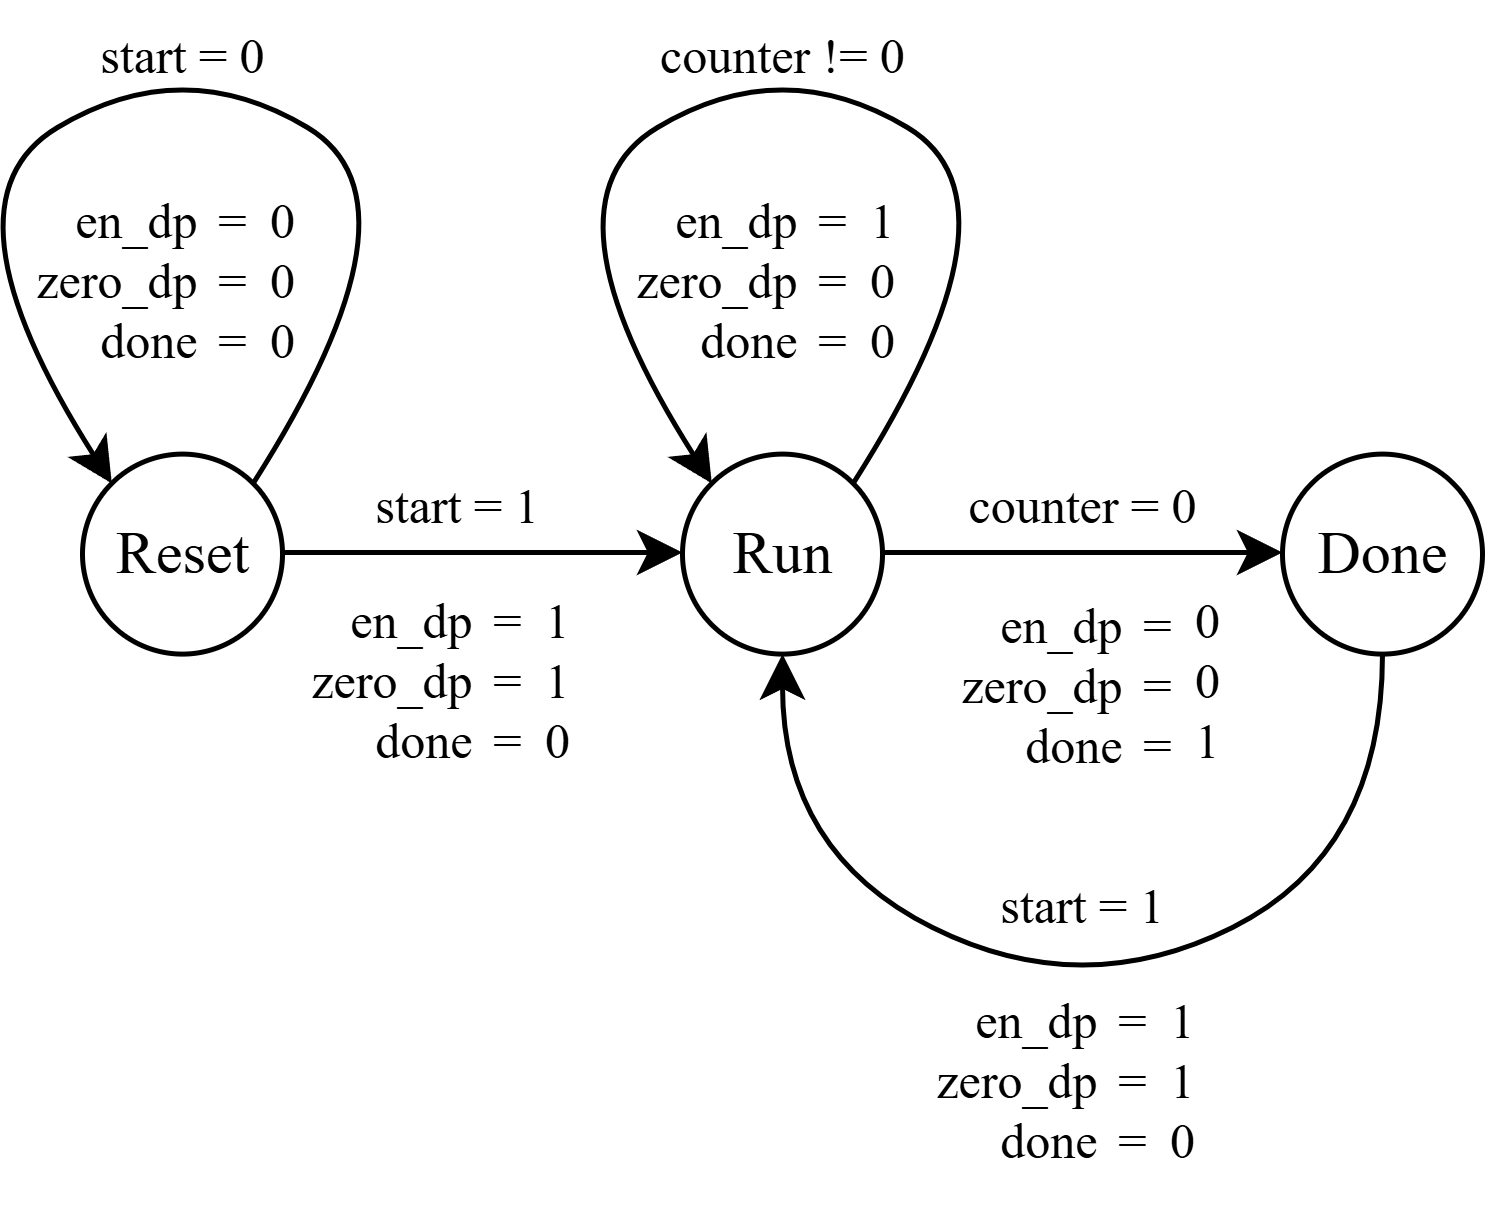
\includegraphics[width=0.8\textwidth]{assets/q4_controller.png}
    \caption{State transitions of the Mealy FSM controller.}
    \label{fig:q4_controller}
\end{figure}

\newpage

\begin{figure}[h]
    \centering
    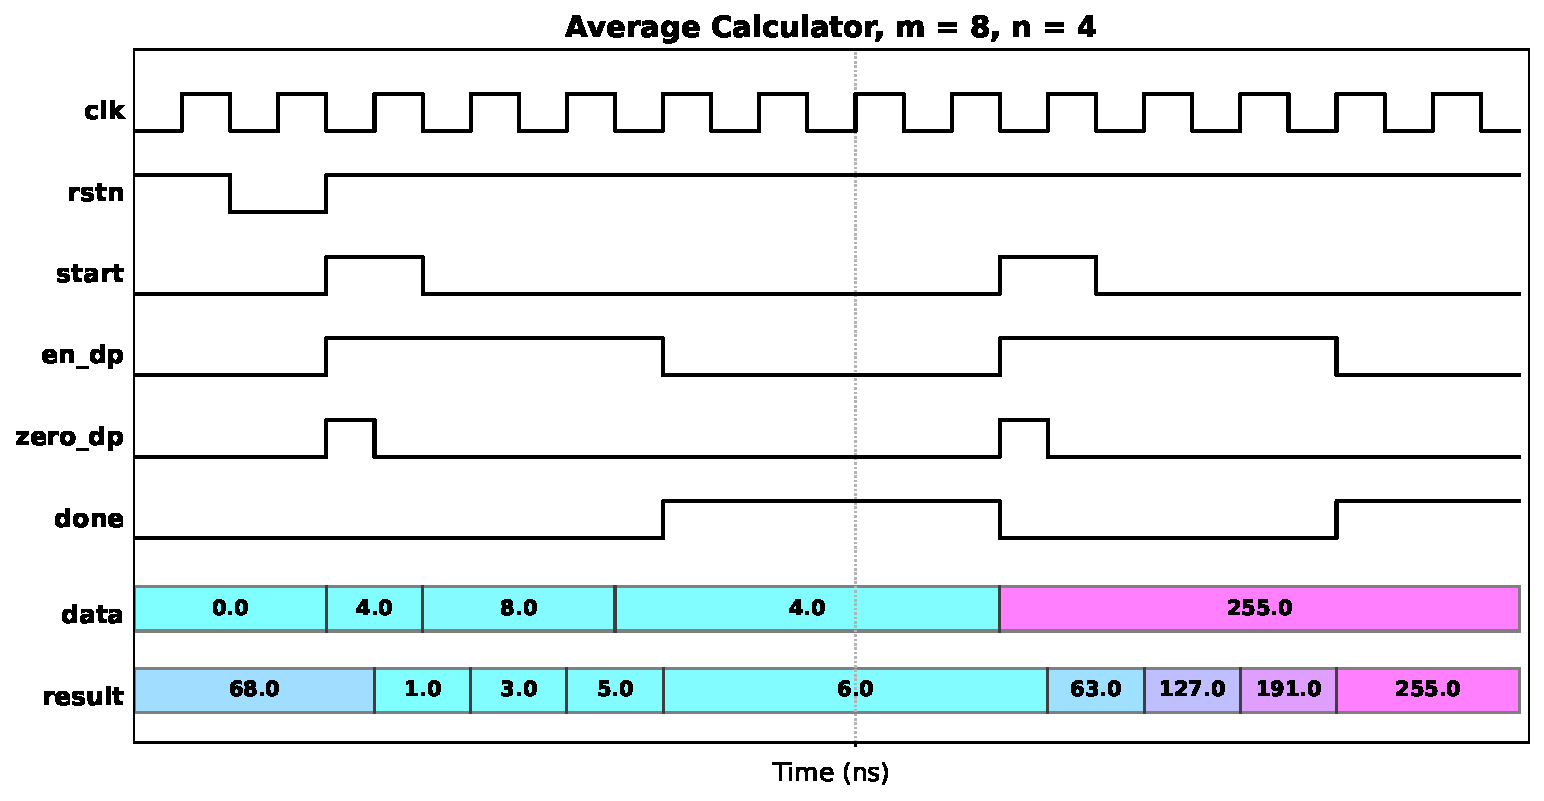
\includegraphics[width=\textwidth]{assets/q4_wave.pdf}
    \caption{Waveforms for the average calculator. Inputs are clocked in on the same cycle as \lstinline{start} is asserted.}
    \label{fig:q4_wave}
\end{figure}

\newpage

\section{Question 5}

The Taylor series expansion of $\sin x$ is shown below.

$$
    \sin(x) = \sum_{n = 0}^\infty \frac{(-1)^n}{(2n+1)!} x^{2n + 1} = x - \frac{x^3}{3!} + \frac{x^5}{5!} - \frac{x^7}{7!} + \frac{x^9}{9!} - \ldots
$$

Design an accelerator that calculates the sin of x based on the Taylor series expansion of sinx. The $x$ signal is a 15-bit fraction and 1-bit integer, $x \in [0, \pi/2]$. The accelerator starts the sin of x when it receives a positive pulse on the \lstinline{start} signal. Accelerator should issue 1 on the \lstinline{done} signal when the result is calculated after eight iterations. The accelerator has a 16-bit fractional output signal called \lstinline{result}, $\text{result} \in [0, 1]$.

\begin{enumerate}
    \item Draw a schematic of your datapath in your report, including the components, interfaces, and necessary control signal. (Use the sin\_coeff\_lut module that is given for the coefficients).
    \item Draw a state diagram that shows the behavior of your controller in your report. In each state, show the control signals that are issued.
    \item Show the wiring between the datapath and controller within the top-level module in your report.
    \item Model the datapath and controller in SystemVerilog.
    \item Model the sinx accelerator by connecting the datapath and controller in SystemVerilog.
    \item Verify the functionality of your accelerator with a testbench.
\end{enumerate}

\subsection*{Solution}

Factorials and exponents are expensive hardware-wise. We start off by determining the recurrence relation of the Taylor series of $\sin x$ to \textit{hopefully} get something more useful for hardware. Each term, $T_n$, in a Taylor series is given by:

$$
T_n = \frac{(-1)^n}{(2n + 1)!} x^{2n + 1}
$$

We can express the next term as follows:

$$
T_{n+1} = \frac{(-1)^{n+1}}{(2n + 3)!} x^{2n + 3}
$$

We are interested in the \textit{relation} between the previous term and the next. We divide:

$$
\frac{T_{n+1}}{T_n} = \frac{(-1)^{n+1}}{(-1)^n} \frac{(2n +1)!}{(2n + 3)!} \frac{x^{2n + 3}}{x^{2n + 1}} = (-1) (x^2) \left( \frac{1}{(2n + 2)(2n + 3)} \right) = - \frac{x^2}{(2n + 2)(2n + 3)}
$$

The final recurrence relation is found by multiplying $T_n$:

$$
T_{n + 1} = - T_n \frac{x^2}{(2n + 2)(2n + 3)}
$$

We now have an expression that is significantly easier to implement in hardware. To further improve performance the fraction is pre-calculated and stored in a Look-Up Table (LUT). The calculations and necessary quantization is done with the following Python script:

\begin{svpython}{Calculation of LUT values}
import math

def quant_15(val):
    return int(round(val * (1 << 15))) & 0xFFFF

val = [1.0]
for i in range(7):
    denom = (2*(i) + 2) * (2*(i) + 3)
    val.append(1 / denom)

for v in val:
    q15 = quant_15(v)
    print(f"{v:.10f} -> 0x{q15:04X}")
\end{svpython}

\begin{textcode}{> python q5\_lut.py}
1.0000000000 -> 0x8000
0.1666666667 -> 0x1555
0.0500000000 -> 0x0666
0.0238095238 -> 0x030C
0.0138888889 -> 0x01C7
0.0090909091 -> 0x012A
0.0064102564 -> 0x00D2
0.0047619048 -> 0x009C
\end{textcode}



\end{document}
